\documentclass[11pt]{article}

\usepackage{amsmath, amssymb}
\usepackage{graphicx}
\usepackage{hyperref}
\usepackage{float}
\usepackage{circuitikz}
\usepackage{tikz}
\usetikzlibrary{arrows.meta}

\title{AC Circuit Modeling}
\author{Mithran Ladhania}
\date{\today}

\begin{document}

\maketitle

\section{Introduction}

This project was assigned on August 21, 2025 as an introductory project during an undergraduate research position at the Bezryadin Lab at Loomis Laboratory, Grainger College of Engineering, University of Illinois Urbana-Champaign.

Resonant circuits, i.e. those circuits incorporating at least one inductive and capacitive element (abbreviated as LC circuits), exhibit oscillatory behavior determined entirely by the values of their components, and form the basis for the frequency-dependent capacitance model which is to be developed later in this project.

\section{Theoretical Background}

\subsection{Overview}

The initial work of this report involved reviewing and re-establishing time-domain circuit theory (for direct current circuits) \cite{uniphysics}. Further, phasor formalism was introduced and reviewed as the base for representing steady-state LC circuits. Further, computational approaches to implementing circuits were analyzed, and the simplest usable one was implemented. 

\subsection{Time-Domain (DC) Model}

The simplest way of representing an LC circuit is through a series circuit of a voltage source ($\epsilon$), an ideal capacitor (capacitance C), and an ideal inductor (inductance L).

% Requires: \usepackage{circuitikz}  in the preamble

\begin{figure}[H]
    \centering
    \begin{circuitikz}[scale=1.2, transform shape]
        \draw
            (0,0) to[battery1, l=$\varepsilon$] (0,3)
            to[short] (3,3)
            to[C, l=$C$] (3,1.5)
            to[L, l=$L$] (3,0)
            to[short] (0,0)
            ;
    \end{circuitikz}
    \caption{Series LC circuit driven by a DC voltage source $\varepsilon$, with capacitance $C$ and inductance $L$.}
    \label{fig:lc_circuit_diagram}
\end{figure}
 

By Kirchhoff's Voltage Law, ``The algebraic sum of the potential differences in any
loop, including those associated with emfs and those of resistive elements, must
equal zero.'' \cite{uniphysics}

We have the following equations for the voltage gain/drop over each component:
$$ V_{\epsilon} = +\epsilon $$
$$ V_{C} = - \frac{q}{C}$$
$$ V_{L} = - L\ddot{q}$$

We can arrange these with KVL to obtain a second order differential equation in $q$. 

$$ \epsilon = \frac{q}{C} + L \ddot{q} $$

\subsubsection{Modelling of a Simple Time-Domain LC Circuit}

Once we have obtained a differential equation that sufficiently describes the time progression of the LC circuit, we can model this behavior with \texttt{scipy}. We turn the second order differential equation into two first order differential equations as follows:

$$ \dot q = i $$
$$ \dot{i} = \frac{\epsilon - {q}/{C}}{L} $$

Defining a state \texttt{S = [q, i]}, which we can plug into \texttt{scipy.integrate}'s \texttt{solve\_ivp}, results for $q(t)$ and $i(t)$ are obtained. The result plotted is as follows:

\begin{figure}[H]
    \centering
    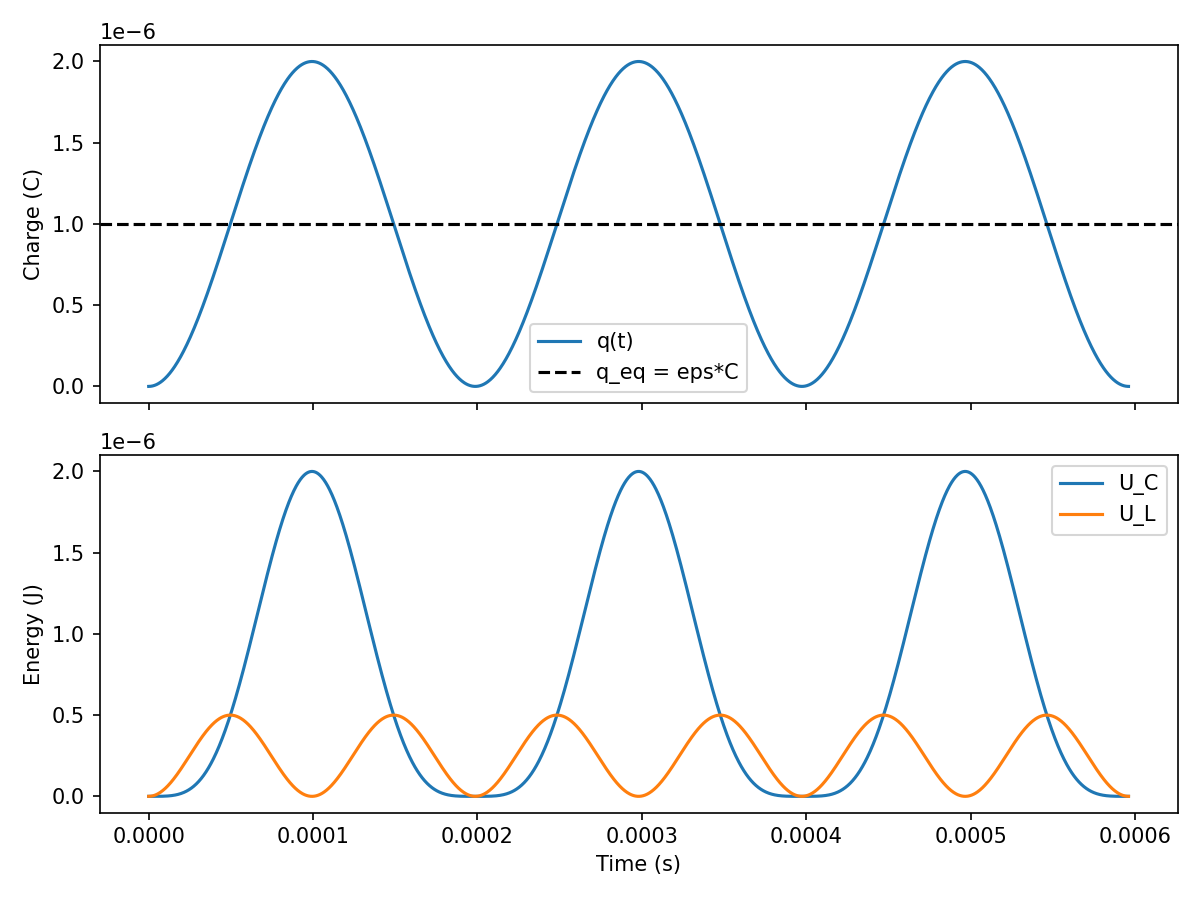
\includegraphics[width=0.8\textwidth]{driven_lc.png}
    \caption{Driven LC circuit response: charge $Q(t)$ (top) oscillates about the equilibrium $Q_{eq} = \varepsilon C$, and the corresponding capacitor and inductor energies $U_C$, $U_L$ (bottom) oscillate with constant amplitudes.}
    \label{fig:driven_lc}
\end{figure}

\subsection{Phasor Formalism and the AC Extension}

As opposed to direct current circuits, which are best represented in the time domain (with time-varying equations for state variables and dynamic quantities), alternating current (ac) circuits in sinusoidal steady state can be best analyzed through complex phasors. There are two main benefits to this approach: (1) a system of differential equations is simplified to an algebraic equation, and (2) addition and subtraction of complex phasors allow circuits to be resolved without arduous sine and cosine additions.

\subsubsection{Phasor Theory}

A complex, rotating phasor is defined as follows:

$$ \tilde{X}(t) = Ae^{i\phi}e^{i \omega t}$$

It is composed of two main parts.

$$\tilde{X} = A\exp({i \phi})$$

$\tilde{X}$ represents the complex amplitude of the phasor, where $A$ is the magnitude/length of the position vector from the center. $\exp(i \phi)$ refers to the phase, or angle from the $\text{Re}$ axis when $t = 0$.

$$\exp(i \omega t)$$

The rotating carrier is a unit rotating vector with an angular frequency of $\omega$. 

The physical quantity represented by a phasor is the real part of the complex signal:
$$ x(t) = \text{Re}\left[\tilde{X} e^{i \omega t}\right] = A\cos(\omega t + \phi)$$

\subsubsection{Single Component AC Circuits}

In this section, we examine how the current phasor $\tilde{I}(t)$ can be obtained for an inductor and a capacitor separately connected to an oscillating voltage.

\textbf{Capacitor}

This setup involves connecting an ideal capacitor of capacitance $C$ to an AC source of peak voltage $\epsilon_0$. 

\begin{figure}[H]
    \centering
    \begin{circuitikz}[scale=0.8, transform shape]
        \draw
            (0,0) to[sV, l=$\varepsilon(t)$] (0,3)
            to[short] (3,3)
            to[C, l=$C$] (3,0)
            to[short] (0,0)
            ;
    \end{circuitikz}
    \caption{Single-element AC circuit: a sinusoidal voltage source $\varepsilon(t)$ driving a capacitor $C$.}
    \label{fig:eps_c_circuit_diagram}
\end{figure}

At a given time $t$, we can state the following fundamental relation for the circuit:

$$ \epsilon (t) = \frac{Q(t)}{C}$$

Our aim is to obtain an expression for the current with respect to time. We can represent $\epsilon(t)$ as the real part of a complex signal:

$$ \epsilon(t) = \text{Re}\left[\tilde{\epsilon}_0 e^{i \omega t}\right] $$

Since $\epsilon(t) = Q(t)/C$ holds for all $t$, and $C$ is a real constant, the same linear relation holds between the corresponding complex representations:

$$ \tilde{\epsilon}(t) = \frac{\tilde{Q}(t)}{C} $$

We know that the real part of the current signal must also be associated with some complex signal $\tilde{I}(t)$. This complex current signal is simply the derivative of the complex charge phasor $\tilde{Q}(t)$, since $I = \dot{Q}$.

Starting from the above-stated capacitor relation in phasor form,
$$ \tilde{\epsilon}_0 e^{i \omega t} = \frac{\tilde{Q}(t)}{C}, $$

we differentiate both sides with respect to $t$:

$$ \frac{d}{dt}\left[\tilde{\epsilon}_0 e^{i \omega t}\right] = \frac{d}{dt}\left[\frac{\tilde{Q}(t)}{C}\right] $$

We get

$$ i\omega \tilde{\epsilon}_0 e^{i \omega t} = \frac{\tilde{I}(t)}{C} $$

so that

$$ \tilde{I}(t) = i\omega C\, \tilde{\epsilon}_0 e^{i \omega t} = i \omega C\, \tilde{\epsilon}(t). $$

Writing $\tilde{I}(t) = \tilde{I}_C\, e^{i\omega t}$ defines the static current phasor $\tilde{I}_C \equiv i\omega C\, \tilde{\epsilon}_0$, which is what is plotted in Figure~\ref{fig:eps_c_phasor_diagram}.

The above equation indicates how the current signal here is different from the voltage signal. First, multiplication by $i$ indicates that the current phasor leads the voltage phasor by $+\pi/2$. Second, the current phasor is scaled by $\omega C$, the susceptance of the capacitor.

\begin{figure}[H]
    \centering
    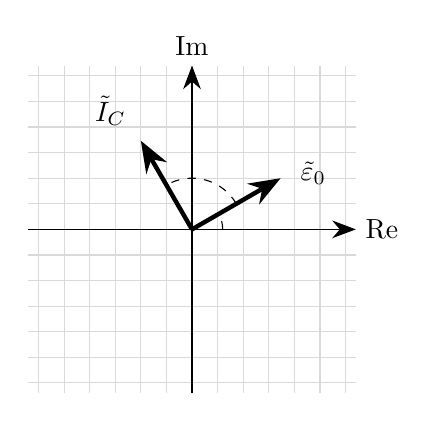
\begin{tikzpicture}[scale=1.3]
        % Square grid background
        \draw[gray!30, step=0.25cm] (-1.6,-1.6) grid (1.6,1.6);

        % Axes, with a serious (Stealth) arrowhead
        \draw[black, -{Stealth[length=3mm]}] (-1.6,0) -- (1.6,0) node[right] {Re};
        \draw[black, -{Stealth[length=3mm]}] (0,-1.6) -- (0,1.6) node[above] {Im};

        % Voltage phasor eps, at phase phi = 30 degrees
        \draw[ultra thick, black, -{Stealth[length=4mm]}] (0,0) -- (0.866,0.5);
        \node[black, right] at (0.966,0.55) {$\tilde{\varepsilon}_0$};

        % Current phasor I_C, at 30 + 90 = 120 degrees
        \draw[ultra thick, black, -{Stealth[length=4mm]}] (0,0) -- (-0.5,0.866);
        \node[black, above left] at (-0.55,0.92) {$\tilde{I}_C$};

        % Angle arcs, dashed, no labels
        \draw[dashed, black] (0.3,0) arc (0:30:0.3);
        \draw[dashed, black] ({0.5*cos(30)},{0.5*sin(30)}) arc (30:120:0.5);
    \end{tikzpicture}
    \caption{Phasor diagram for the eps-C circuit: the current phasor $\tilde{I}_C$ leads the voltage phasor $\tilde{\varepsilon}_0$ by $\pi/2$.}
    \label{fig:eps_c_phasor_diagram}
\end{figure}

\textbf{Inductor}

This setup involves connecting an ideal inductor of inductance $L$ to an AC source of peak voltage $\epsilon_0$.

\begin{figure}[H]
    \centering
    \begin{circuitikz}[scale=0.8, transform shape]
        \draw
            (0,0) to[sV, l=$\varepsilon(t)$] (0,3)
            to[short] (3,3)
            to[L, l=$L$] (3,0)
            to[short] (0,0)
            ;
    \end{circuitikz}
    \caption{Single-element AC circuit: a sinusoidal voltage source $\varepsilon(t)$ driving an inductor $L$.}
    \label{fig:eps_l_circuit_diagram}
\end{figure}

At a given time $t$, we can state the following fundamental relation for the circuit:

$$ \epsilon(t) = L \dot{I}(t) $$

Our aim is to obtain an expression for the current with respect to time. We can represent $\epsilon(t)$ as the real part of a complex signal:

$$ \epsilon(t) = \text{Re}\left[\tilde{\epsilon}_0 e^{i \omega t}\right] $$

Since $\epsilon(t) = L\dot{I}(t)$ holds for all $t$, and $L$ is a real constant, the same linear relation holds between the corresponding complex representations:

$$ \tilde{\epsilon}(t) = L \frac{d\tilde{I}(t)}{dt} $$

We know that the real part of the current signal must also be associated with some complex signal $\tilde{I}(t)$. Unlike the capacitor case, where the current phasor was obtained by differentiating the charge phasor, here the current phasor must be obtained by integrating the voltage phasor, since $I(t) = \frac{1}{L}\int \epsilon(t) \, dt$.

Starting from the inductor relation in phasor form,
$$ \tilde{\epsilon}_0 e^{i \omega t} = L \frac{d\tilde{I}(t)}{dt}, $$

we integrate both sides with respect to $t$:

$$ \int \tilde{\epsilon}_0 e^{i \omega t} \, dt = \int L \frac{d\tilde{I}(t)}{dt} \, dt $$

We get

$$ \frac{\tilde{\epsilon}_0}{i\omega} e^{i \omega t} = L\, \tilde{I}(t) $$

so that

$$ \tilde{I}(t) = \frac{\tilde{\epsilon}_0}{i \omega L} e^{i \omega t} = \frac{\tilde{\epsilon}(t)}{i \omega L}. $$

(The constant of integration corresponds to a non-oscillating offset, and is neglected here, since we are only concerned with the steady-state phasor representation.)

Writing $\tilde{I}(t) = \tilde{I}_L\, e^{i\omega t}$ defines the static current phasor $\tilde{I}_L \equiv \dfrac{\tilde{\epsilon}_0}{i \omega L}$, which is plotted in Figure~\ref{fig:eps_l_phasor_diagram}.

The above equation indicates how the current signal here is different from the voltage signal. First, division by $i$ indicates that the current phasor lags the voltage phasor by $\pi/2$ (the opposite of the capacitor case). Second, the current phasor is scaled by $\frac{1}{\omega L}$; the susceptance of the inductor is $B_L = -\frac{1}{\omega L}$, negative rather than positive as in the capacitor case, reflecting this lag.

\begin{figure}[H]
    \centering
    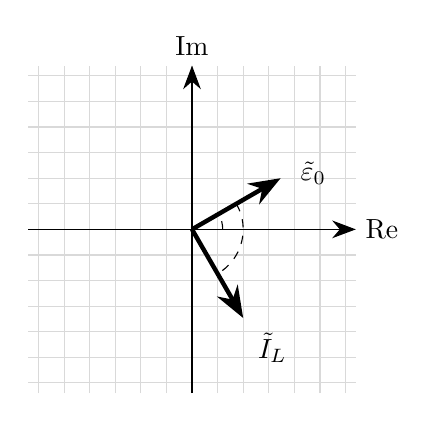
\begin{tikzpicture}[scale=1.3]
        % Square grid background
        \draw[gray!30, step=0.25cm] (-1.6,-1.6) grid (1.6,1.6);

        % Axes, with a serious (Stealth) arrowhead
        \draw[black, -{Stealth[length=3mm]}] (-1.6,0) -- (1.6,0) node[right] {Re};
        \draw[black, -{Stealth[length=3mm]}] (0,-1.6) -- (0,1.6) node[above] {Im};

        % Voltage phasor eps, at phase phi = 30 degrees
        \draw[ultra thick, black, -{Stealth[length=4mm]}] (0,0) -- (0.866,0.5);
        \node[black, right] at (0.966,0.55) {$\tilde{\varepsilon}_0$};

        % Current phasor I_L, at 30 - 90 = -60 degrees
        \draw[ultra thick, black, -{Stealth[length=4mm]}] (0,0) -- (0.5,-0.866);
        \node[black, below right] at (0.55,-0.92) {$\tilde{I}_L$};

        % Angle arcs, dashed, no labels
        \draw[dashed, black] (0.3,0) arc (0:30:0.3);
        \draw[dashed, black] ({0.5*cos(30)},{0.5*sin(30)}) arc (30:-60:0.5);
    \end{tikzpicture}
    \caption{Phasor diagram for the eps-L circuit: the current phasor $\tilde{I}_L$ lags the voltage phasor $\tilde{\varepsilon}_0$ by $\pi/2$.}
    \label{fig:eps_l_phasor_diagram}
\end{figure}

\subsection{Inductor-Capacitor AC Circuit}

This setup connects the capacitor of capacitance $C$ and the inductor of inductance $L$ in series to an AC source of peak voltage $\epsilon_0$. 

% Requires: \usepackage{circuitikz}  in the preamble

\begin{figure}[H]
    \centering
    \begin{circuitikz}[scale=0.8, transform shape]
        \draw
            (0,0) to[sV, l=$\varepsilon(t)$] (0,3)
            to[short] (3,3)
            to[C, l=$C$] (3,1.5)
            to[L, l=$L$] (3,0)
            to[short] (0,0)
            ;
    \end{circuitikz}
    \caption{Series LC circuit driven by an AC voltage source $\varepsilon(t)$, with capacitance $C$ and inductance $L$ sharing a single loop current $I(t)$.}
    \label{fig:lc_ac_circuit_diagram}
\end{figure}

As established in the above sections, we can state the following fundamental relation for the circuit:

$$\epsilon(t) = V_L(t) + V_C(t) = \frac{Q(t)}{C} + L\dot{I}(t)$$

To obtain an expression for the current as a function of time, we can again represent $\epsilon(t)$ as the real part of the complex signal. We can express the combined effect of the capacitor and inductor by adding the individual signals from the capacitor and inductor as phasors.

We can first express each voltage drop as a phasor:

$$ \tilde{V}_L(t) = i\omega L\, \tilde{I}(t), \qquad \tilde{V}_C(t) = \frac{\tilde{I}(t)}{i\omega C} $$

We can substitute these into the KVL relation

$$ \tilde{\epsilon}(t) = \tilde{I}(t)\left(i\omega L + \frac{1}{i\omega C}\right) $$

This bracketed quantity is the total impedance of this circuit. 

$$ Z(\omega) = i\omega L + \frac{1}{i\omega C}, $$

so that the loop current phasor is
 
$$ \tilde{I}(t) = \frac{\tilde{\epsilon}(t)}{Z(\omega)}. $$

Since $Z(\omega)$ is purely imaginary for all $\omega$ -- there being no resistive element in this circuit -- the current phasor is always exactly $\pm\pi/2$ out of phase with the voltage phasor, never any angle in between; which of the two signs applies depends on whether $\omega L$ or $1/(\omega C)$ dominates at a given frequency. The magnitude of the current is set by $|Z(\omega)|$, and vanishes entirely at the resonant frequency $\omega_0 = 1/\sqrt{LC}$, where $\text{Im}[Z(\omega)] = 0$ and the capacitive and inductive contributions cancel exactly.

\section{Computational Implementation}

\subsection{Architecture}

Phasor formalism developed above is implemented directly in Python, with a \texttt{Phasor} class representing the static complex phasor $\tilde{X} = Ae^{i\phi}$ at a fixed angular frequency $\omega$. The class stores only these three quantities (amplitude, phase and frequency) as instance variables. Time and any derived complex value are computed on demand, since they are properties of a specific query and cannot be considered properties of the phasor itself.

\texttt{Phasor} has four methods:

\begin{itemize}
    \item \texttt{snapshot()} returns the static complex value $Ae^{i\phi}$.
    \item \texttt{at(t)} returns the full time-dependent signal $\tilde{X}e^{i\omega t}$, for a scalar or array \texttt{t}.
    \item \texttt{signal(t)} returns the physical, real-valued signal $\text{Re}[\tilde{X}e^{i\omega t}]$.
    \item \texttt{dif\_t()} and \texttt{int\_t()} return new \texttt{Phasor} objects corresponding to the derivative and integral of the signal, matching the amplitude-scaling and phase-shift relations derived above for the capacitor and inductor cases. Since differentiation and integration of a phasor return another phasor at the same $\omega$, both methods are closed under the \texttt{Phasor} type -- a differentiated phasor can itself be differentiated, or evaluated at a time \texttt{t}.
\end{itemize}

\texttt{int\_t()} raises an explicit error when $\omega = 0$, since a DC phasor has no bounded phasor representation of its integral.

Four circuit classes are built on top of \texttt{Phasor}:

\begin{itemize}
    \item \texttt{VoltageSource} wraps a single \texttt{Phasor} representing $\tilde{\epsilon}(t)$.
    \item \texttt{Capacitor} takes a \texttt{VoltageSource} and a capacitance value, and computes the resulting current phasor directly from \texttt{dif\_t()}, scaled by $C$.
    \item \texttt{Inductor} takes a \texttt{VoltageSource} and an inductance value, and computes the resulting current phasor directly from \texttt{int\_t()}, scaled by $1/L$.
    \item \texttt{LCCircuit} does not reuse \texttt{Capacitor} or \texttt{Inductor}, since both of those classes assume they are the only element across the source. Instead, \texttt{LCCircuit} computes $Z_L$ and $Z_C$ directly as plain complex numbers, sums them into $Z_{total}$, and solves $\tilde{I} = \tilde{\epsilon}/Z_{total}$ per the KVL relation derived above. Impedance is not represented as a \texttt{Phasor}, since it is a frequency-dependent constant rather than an oscillating signal.
\end{itemize}

For visualization, each phasor's rotation is drawn on a complex plane using its \texttt{at(t)} values, and the corresponding real signal is plotted from \texttt{signal(t)}. A slider control was used in place of a frame-by-frame animation, allowing the circuit's state to be inspected at any point in time without re-running a simulation loop.

\subsection{Validation}

The capacitor and inductor implementations were checked against the closed-form results derived by hand above for each single-element case. With $\epsilon_0 = \omega = C = L = 1$, both the amplitude and phase of the current phasors \texttt{Capacitor.I} and \texttt{Inductor.I} matched the predicted values of $1.0$ and $\pm\pi/2$ exactly, confirming that \texttt{dif\_t()} and \texttt{int\_t()} correctly applied amplitude scaling as well as phase shift.

The combined \texttt{LCCircuit} was checked by confirming $Z(\omega)$ is purely imaginary for all tested values of $L$, $C$, and $\omega$, consistent with the absence of a resistive element, and by confirming that the current phasor's phase is always exactly $\pm\pi/2$ relative to the source, never any intermediate angle. The resonance condition $\omega_0 = 1/\sqrt{LC}$ was also verified directly against $Z_{total}$, confirming $|Z_{total}| \to 0$ as $\omega \to \omega_0$.

\subsection{Frequency-Dependent Capacitance}

This will extend the circuit model above by allowing the capacitance to become a complex, frequency-dependent quantity $C(\omega)$, following the Debye relaxation framework, and will require both a review of the relevant dielectric relaxation literature and an extension of the existing computational implementation.

\bibliographystyle{plain}
\bibliography{references}

\end{document}